\documentclass[12pt,a4paper]{article}
% The following LaTeX packages must be installed on your machine: amsmath, authblk, bm, booktabs, caption, dcolumn, fancyhdr, geometry, graphicx, hyperref, latexsym, natbib
\input{151.dat}
\usepackage{gensymb}
\usepackage{float}
\usepackage{siunitx}
\usepackage{amssymb}
\usepackage{float}
\usepackage{enumerate}
\usepackage{listings}
\PassOptionsToPackage{hyphens}{url}\usepackage{hyperref}
\usepackage[none]{hyphenat}
%\renewcommand{\familydefault}{\sfdefault}


\begin{document}

\setcounter{page}{1}

\section*{Problem 2.8}

\begin{figure}[htb]
	\centering
	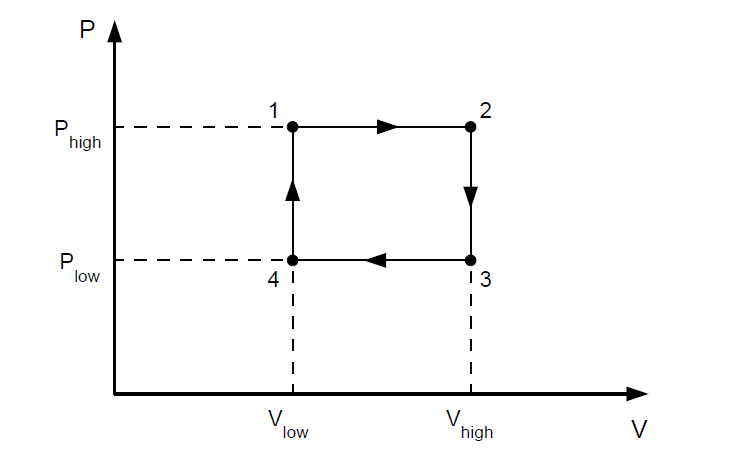
\includegraphics[width=0.8\textwidth]{work.png}
	\caption{Cyclic process for this problem.}
	\label{fig:cycle}
\end{figure}

\begin{enumerate}[(a)]

\item The net work done on the system (traversing the path codirectional with the arrows) is nonzero since it depends on the initial and final macrostates, sa well as the intermediate macrostates (i.e. the path).

\item If the work done followed a path $1 \rightarrow 2 \rightarrow 3 \rightarrow 1$ all in straight lines, then it would be equal to the negative of half the area of the original rectangular path.

\end{enumerate}

\end{document}